\chapter{Estruturas Condicionais}
\section{Condições}
Em alguns algoritmos, como os vistos no capítulo anterior, a execução se dá de maneira pré-definida, porém estruturas condicionais servem para modificar o fluxo do algoritmo, como decidir se deve ser utilizado o bloco de instruções A ou B, vide Figura \ref{fig:fluxo}.
\begin{figure}[!h]
    \centering
    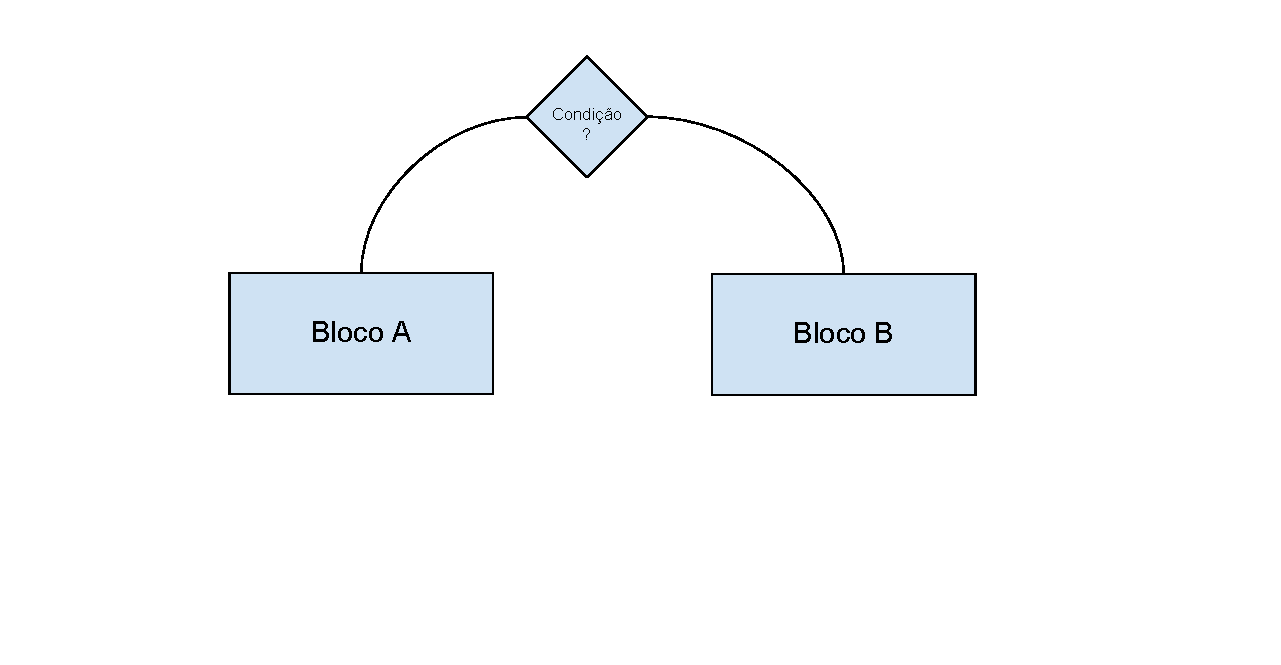
\includegraphics[scale=.5]{condicional.pdf}
    \caption{Fluxograma condicional}
    \label{fig:fluxo}
\end{figure}
Basicamente uma pergunta que deve ser respondida com os tipos lógicos Verdadeiro ou Falso, e pode ser utilizado em conjunto com os operadores lógicos, alguns presentes na tabela \ref{tab:operadoresLogicos}.
\begin{table}[!h]
\centering
\caption{Operadores lógicos}
\label{tab:operadoresLogicos}
\begin{tabular}{cc} \hline \hline
Operador      & Definição          \\ \hline
\&\&          & E                  \\
||            & OU                 \\
!             & Negação            \\
\textgreater  & Maior que          \\
\textgreater= & Maior ou igual que \\
\textless     & Menor que          \\
\textless=    & Menor ou igual que \\ \hline \hline

\end{tabular}
\end{table}

As estruturas condiconais podem ser simples ou compostas, a seguir têm-se o funcionamento das duas estruturas, começando pela simples.
\begin{lstlisting}
    Se <condicao> entao
        <comando1>
        <comando2>
        .
        .
        .
        <comandoN>
    Fim-Se
\end{lstlisting}
\textbf{Exemplo:} \textbf{Se} um cliente queira que suas compras sejam embrulhadas para presente deverá pagar uma taxa adicional de R\$$3,50$. Logo, para calcular o preço total deve-se saber se a mercadoria deve ser embrulhada.
\begin{lstlisting}
    valor: real
    presente: caracter
    Escreva("Informe o valor da mercadoria: ")
    Leia(valor)
    Escreva("Deseja embrulhar para presente?")
    Leia(presente)
    Se presente == 'S' entao
        valor = valor + 3.5
    Fim-Se
    Escreva("Total a pagar : " + valor)
\end{lstlisting}
Note que caso a informação guardada na variável presente for equivalente ao caracter 'S' então o valor da compra terá um acréscimo referente ao valor do embrulho. \\
Para as estruturas compostas temos a adição de duas novas palavras reservadas: o senão e o senão-se. Que servem para o caso contrário da condição, ou para condições extras, por exemplo: \\
Dados três números distintos, elabore um algoritmo que escreva o maior número digitado.
\begin{lstlisting}
    a,b,c: inteiro
    Leia(a, b, c)
    Se (A>B) entao
        Se (A>C) entao
            Escreva("O maior numero e A")
        Fim-Se
    Senao
        Se (B>C) entao
            Escreva("O maior numero e B")
        Senao
            Escreva("O maior numero e C")
        Fim-se
    Fim-Se
\end{lstlisting}
Note que o senão não precisa de condição, pois utiliza o contrário da condição do Se anterior. Podemos melhorar o algoritmo acima utilizando o senão se:
\begin{lstlisting}
    a,b,c: inteiro
    Leia(a, b, c)
    Se (A>B) E (A>C) entao
        Escreva("O maior numero e A")
    Senao Se (B>C) entao
        Escreva("O maior numero e B")
    Senao
        Escreva("O maior numero e C")
    Fim-Se
\end{lstlisting}
Isto funciona pois utiliza-se o operador lógico E na condição, logo se A>B e A>C, o A é o maior. Porém se falhar na condição de A>B, temos de testar B>C para decidir qual dos outros será o maior. Note também que podemos fazer estrutras condicionais equivalentes utilizando o operador lógico da negação (!).
\begin{lstlisting}
    Se <condicao> entao
        <comandos1>
    Senao
        <comandos2>
    Fim-se
\end{lstlisting}
\begin{lstlisting}
    Se !<condicao> entao
        <comandos2>
    Senao
        <comandos1>
    Fim-se
\end{lstlisting}
As duas estruturas se tornam equivalentes, pois inverte-se a ordem em que os comandos serão dados, na primeira estrutura os comandos1 vão ser executados, já na segunda os comandos2.